\section{Diffraction de la lumière par un réseau et interférences}

Que se passera-t-il si nous utilisons plusieurs fentes (appelé réseau)
au lieu de deux comme dans l'expérience de Young~?

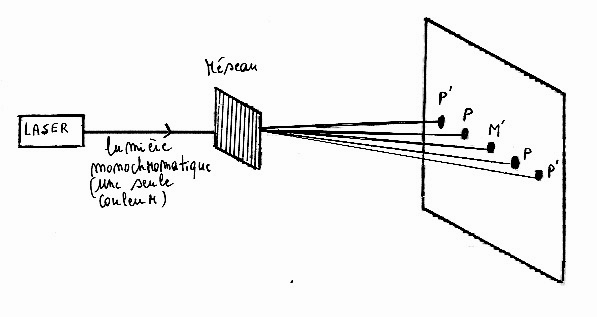
\includegraphics[width=8.565cm,height=4.546cm]{Pictures/10000001000002550000013DE02531D3FDE95D32.png}

Un réseau de diffraction est constitué d'un très grand nombre de fentes,
(au lieu de deux dans l'expérience de Young), très fines et très proches
les unes des autres, parallèles et équidistantes.

La distance entre deux fentes est $a$.

Si de la lumière provenant du laser est une lumière monochromatique (une
seule couleur et donc une seule fréquence), il apparaît alors sur
l'écran une série de points lumineux~: un point central M' dans le
prolongement du faisceau incident et des points lumineux, P,P',\ldots{}
répartis symétriquement de part et d'autre du point central.

Nous observons donc une figure d'interférences, comme dans le cas de
l'expérience de Young.

Cherchons une relation entre $i, \lambda, a et D.$

\begin{figure}
\centering
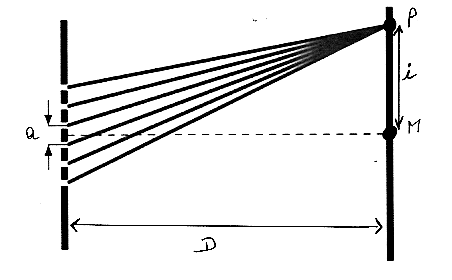
\includegraphics[width=7.086cm,height=4.389cm]{Pictures/10000001000001C400000118A4F6B6134DC391C7.png}
\caption{}
\end{figure}

Chaque fente étant très étroite, il y a une diffraction importante~: on
pet donc considérer que chaque fente se comporte comme une nouvelle
source d'ondes circulaires envoyant des ondes dans toutes les
directions. Par clarté, nous ne dessinerons que celle qui atteignent un
point P.

Ces ondes venant de chacune des fentes vont interférer.

On constate que les distances des très nombreuses fentes au point P sont
très légèrement différentes, ce qui entraine un déphasage des
différentes ondes arrivant au point P.

\begin{figure}
\centering
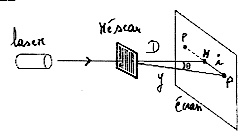
\includegraphics[width=8.348cm,height=4.235cm]{Pictures/10000001000000F800000088FE88597F2483A271.png}
\caption{}
\end{figure}

M est le point lumineux central,

P les points lumineux consécutifs au point central.

Nous pouvons mesurer~:
\begin{description}
	\item[$i$] l'interfrange,
	\item[$\theta$] l'angle de déviation,
	\item[$D$] distance entre le réseau et l'écran.
\end{description}

Ceci nous permettra de calculer la longueur d'onde de la lumière.

La relation entre $\lambda, i, a$ et $D$ est FIXME

\begin{figure}
\centering
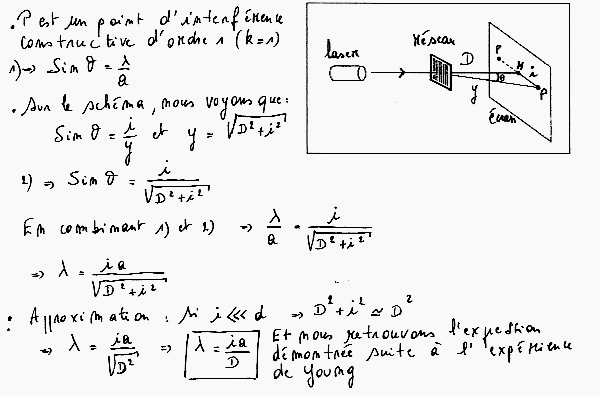
\includegraphics[width=19.177cm,height=12.658cm]{Pictures/10000001000002580000018C86EAAA8910282BD9.png}
\caption{}
\end{figure}

\subsection{Synthèse}

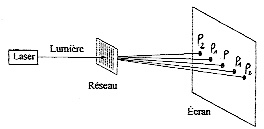
\includegraphics[width=8.976cm,height=4.397cm]{Pictures/100000010000010800000081DE709BA3D328A388.png}
\includegraphics[width=1.757cm,height=1.432cm]{Pictures/100000010000001A0000001535F2FEA5DABE5CC8.png}

\subsection{Exercices}

\subsubsection{Ex. 1}

Un réseau a 300 fentes/mm. On fait passer de la lumière rouge ayant une
longueur d'onde de 650 nm dans le réseau et on observe les maximums sur
un écran situé à 2,4 m du réseau.

Quelle est la distance sur l'écran entre le maximum d'ordre 1 et le
maximum central? (Rép~: 468 mm)

\subsubsection{Ex. 2}

De la lumière de longueur d'onde égale à 550 nm éclaire selon la normale
un réseau comprenant 400 traits par mm. Calcule l'angle sous lequel on
observe les maxima pour les ordres 2 et 3.
(Rép~: 26° et 41,3°)

\subsubsection{Ex. 3}

On fait passer de la lumière provenant d'une ampoule au sodium à travers
un réseau ayant 300 fentes/mm. On observe les maximums sur un écran
situé à 2 m des fentes. Dans la lumière faite par une telle lampe, on
retrouve de la lumière ayant une longueur d'onde de 589,0 nm et de la
lumière ayant une longueur d'onde de 589,6 nm (qu'on appelle le doublet
du sodium). Quelle est la distance sur l'écran entre les maximums
d'ordre 1 de ces deux ondes de longueurs d'onde différente?
(Rép~: 0,36 mm)

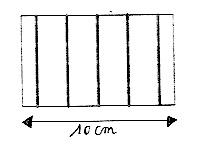
\includegraphics[width=5.008cm,height=3.551cm]{Pictures/10000001000000C70000008D88834268E2E16F18.png}

\subsubsection{Ex. 4}

Sur un écran situé à 46 cm d'un réseau éclairé avec de la lumière
monochromatique, on observe la figure suivante : Le pas du réseau est de
10 μ m.

\begin{enumerate}
\item  En déduire la longueur d'onde de la lumière monochromatique qui
  éclaire le réseau. (Rép~: 435 nm)
\item  De quelle couleur s'agit-il ? (Rép~: bleu)
\end{enumerate}

\subsection{Résolutions}

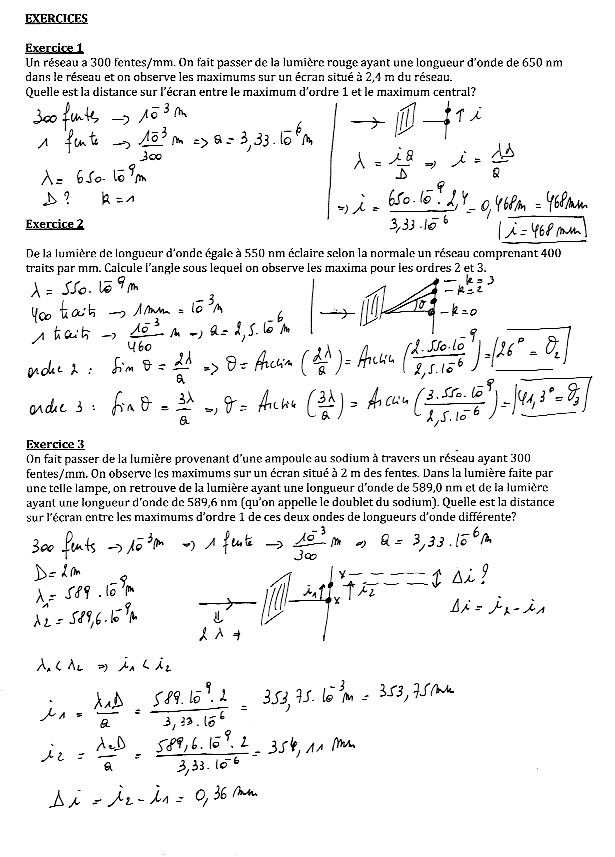
\includegraphics[width=18.503cm,height=25.788cm]{Pictures/1000000100000267000003591812743A6BDA8B59.png}

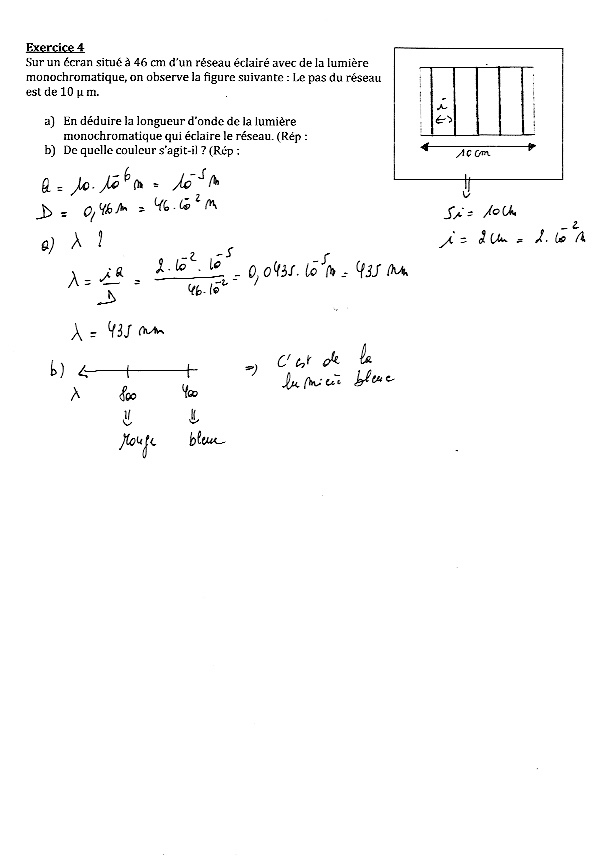
\includegraphics[width=18.503cm,height=25.788cm]{Pictures/100000010000026700000359459F0C15512CA66D.png}
